\begin{titlepage}
\newcommand{\HRule}{\rule{\linewidth}{0.5mm}} % Defines a new command for the horizontal lines, change thickness here
\centering % Center everything on the page
 
%	HEADING SECTIONS
\null
\vspace{1cm}
\textsc{\Large Université Catholique de Louvain}\\[1cm] % Name of your university/college
\textsc{\large MECA2170 \\[0.3cm] Numerical Geometry}\\[0.5cm] % Major heading such as course name
%\textsc{\large Minor Heading}\\[0.5cm] % Minor heading such as course title

%	TITLE SECTION

\HRule \\[0.4cm]
{ \LARGE \bfseries Delaunay's triangulation\\[0.4cm] % Title of your document
\large \bfseries Report} \\[0.4cm]

\HRule \\[0.5cm]
 
\begin{figure}[!h]
	\begin{center}
	%2048 × 1364
		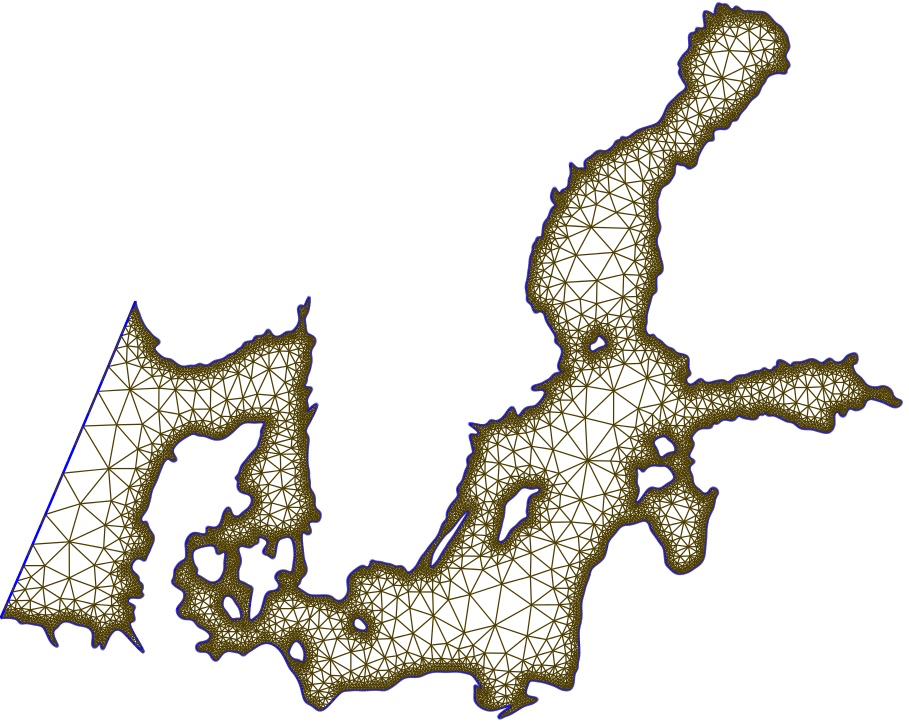
\includegraphics[width=10.5cm]{images/cover.jpg}
	\end{center}
\end{figure}

%	AUTHOR SECTION

\large 
\centering
{\begin{tabular}{lll}
\textsc{CERCKEL} & Arnaud\\
\textsc{STEVENS} & Nicolas\\
\end{tabular}}
\\[1cm]

\normalsize
{\begin{tabular}{ll}
\textit{Professeurs} : & Vincent Legat \& Jean François Remacle\\
\end{tabular}}
\\[1cm]

%	DATE SECTION

{\normalsize \today}\\[2cm] % Date, change the \today to a set date if you want to be precise

\end{titlepage}
\newpage